%\documentclass[fleqn]{article}
\documentclass[nocopyrightspace]{sigplanconf}

\usepackage{xspace,pads,amsmath,math-cmds,
            math-envs,inference-rules,times,
            verbatim,alltt,multicol,proof,url}

\usepackage{code} 
\usepackage{epsfig}


%\setlength{\oddsidemargin}{0in}
%\setlength{\evensidemargin}{0in}
%\setlength{\textwidth}{6.5in}
%\setlength{\textheight}{8.5in}

\begin{document}
\title{Fully Automatic Tool Generation for Ad Hoc Data}

\authorinfo{Kathleen Fisher}{
	   AT\&T Labs Research}
       {\mono{kfisher@research.att.com}}
\authorinfo{David Walker}{
	   Princeton University}
       {\mono{dpw@CS.Princeton.EDU}}
\authorinfo{Peter White}{
	   Galois Connections}
       {\mono{peter@galois.com}}
\authorinfo{Kenny Q. Zhu}{
	   Princeton University}
       {\mono{kzhu@CS.Princeton.EDU}}
\newcommand{\cut}[1]{}
\newcommand{\reminder}[1]{{\it #1 }}
\newcommand{\poplversion}[1]{#1}
\newcommand{\trversion}[1]{}

\newcommand{\appref}[1]{Appendix~\ref{#1}}
\newcommand{\secref}[1]{Section~\ref{#1}}
\newcommand{\tblref}[1]{Table~\ref{#1}}
\newcommand{\figref}[1]{Figure~\ref{#1}}
\newcommand{\listingref}[1]{Listing~\ref{#1}}
%\newcommand{\pref}[1]{{page~\pageref{#1}}}

\newcommand{\eg}{{\em e.g.}}
\newcommand{\cf}{{\em cf.}}
\newcommand{\ie}{{\em i.e.}}
\newcommand{\etc}{{\em etc.\/}}
\newcommand{\naive}{na\"{\i}ve}
\newcommand{\role}{r\^{o}le}
\newcommand{\forte}{{fort\'{e}\/}}
\newcommand{\appr}{\~{}}

%\newcommand{\bftt}[1]{{\ttfamily\bfseries{}#1}}
\newcommand{\kw}[1]{\bftt{#1}}
\newcommand{\pads}{\textsc{pads}}
\newcommand{\padsc}{\textsc{pads/c}}
\newcommand{\ipads}{\textsc{ipads}}
\newcommand{\padsl}{\textsc{padsl}}
\newcommand{\blt}{\textsc{blt}}
\newcommand{\ddc}{\textsc{ddc}$^{\alpha}$}
\newcommand{\ddcold}{\textsc{ddc}}
\newcommand{\padsml}{\textsc{pads/ml}}
\newcommand{\padsmlbig}{\textsc{PADS/ML}}
\newcommand{\ddl}{\textsc{ddl}}
\newcommand{\C}{\textsc{c}}
\newcommand{\perl}{\textsc{perl}}
\newcommand{\ml}{\textsc{ml}}
\newcommand{\smlnj}{\textsc{sml/nj}}
\newcommand{\ocaml}{\textsc{o'caml}}
\newcommand{\java}{\textsc{java}}
\newcommand{\xml}{\textsc{xml}}
\newcommand{\xquery}{\textsc{xquery}}
\newcommand{\datascript}{\textsc{datascript}}
\newcommand{\packettypes}{\textsc{packettypes}}
\newcommand{\erlang}{\textsc{Erlang}}

\newcommand{\dibbler}{Sirius}
\newcommand{\ningaui}{Altair}
\newcommand{\darkstar}{Regulus}

%% \newcommand{\IParray}[4]{{\tt Parray} \; #1 \; \[#2, #3, #4\]}

\newcommand{\figHeight}[4]{\begin{figure}[tb]
	\centerline{
	            \epsfig{file=#1,height=#4}}
	\caption{#2}
	\label{#3}
	\end{figure}}


\maketitle{}

\begin{abstract}  
Many applications use the file system as a simple persistent data
store.  This approach is expedient, but it is not robust.  In general,
the overall correctness of such an application dependso on the
collection of files, directories, and symbolic links having some
precise hierarchical organization. Furthermore file system properties
such as file ownership, permissions, and timestamps must have
acceptable values. Unfortunately, current programming languages do not
provide support for documenting assumptions about the file system. In
addition, actually loading data from disk requires writing tedious
boilerplate code.

This paper describes \forest{}, a new domain-specific language for
describing directory structures embedded in \haskell{}. \forest{}
descriptions use a type-based metaphor to specify portions of the file
system in a simple, declarative manner.  \forest{} makes it easy to
connect data on disk to an isomorphic representation in memory
that can be manipulated by programmers as if it were any other
data structure in their program.  \forest{} generates
metadata that describes to what degree the files on disk conform to
the specification, making error detection easy. The system greatly
lowers the divide between on-disk and in-memory representations of
data. \forest{} leverages \haskell{}'s powerful generic programming
infrastructure to make it easy for third-party developers to build
tools that work for any \forest{} description.  We illustrate the use
of this infrastructure to build a number of useful tools, including a
visualizer, permission checker, and description-specific tools for a
number of standard shell tools.

\cut{
We present the design for \forest{} and describe the implementation of
a full working prototype. From a single compact description, the
\forest{} compiler generates a collection of \haskell{} types and
functions for validating and analyzing file system data.  In addition,
\forest{} generates type class instance declarations that make it
possible to exploit powerful generic programming paradigms that allow
third-party developers to build tools for querying, visualizing, and
debugging on-disk data in a generic way. We present examples
illustrating the use of \forest{} on a number of real-world directory
structures and programming tasks, including description-specific
replacements for a number of standard shell tools. Finally, we
formalize the core elements of the language as a simple calculus based
on classical tree logics.}
\end{abstract}

\section {Introduction}
\label{sec:intro}
\section{Introduction}
\label{sec:intro}

\datascript{}~\cite{gpce02}. \packettypes{}~\cite{sigcomm00}. \padsc{}~\cite{fisher+:pads}
and \padsml{}~\cite{mandelbaum+:padsml}. Bro\cite{paxson:bro}. These
are but a few of the many languages designed for describing data
formats. In his classic paper {\em The Next 700 Programming
  Languages}, 1966~\cite{landin:700}, Landin asserts that principled
programming language design involves thinking in terms of ``families
of languages'' and choosing from a ``well-mapped space.''  However,
when it comes to the domain of processing ad hoc data, there is no
well-mapped space and no systematic understanding of the family of
languages one might be dealing with.

In our previous work, we developed the data description calculus
\ddcold{} to capture the core features of many existing data
description languages~\cite{fisher+:next700ddl}, like \padsc{},
\packettypes{} and \datascript{}. Given the broad applicability of
\ddcold{}, we wanted to use it to define the semantics of
\padsml{}. However, the polymorphic types that we wished to include in
\padsml{} can not be formalized with \ddcold{}.  In addition, both
\padsc{} and \padsml{} generate tools from data format descriptions to
{\em print} data in the specified format. For
many applications, printing data correctly can be as important as
parsing it correctly. Yet, our previous work
specified only the type and parsing semantics of \ddcold{}. 

In this work, we address both of these limitations of
\ddcold{}. First, we extend \ddcold{} with abstractions over types to
create \ddc. In the process, we also improve the \ddc\ theory, as
noted in \secref{sec:ddc-sem}. The new \ddc provides basis for
specifying the semantics of \padsml{}. Second, we specify the a
printing semantics for the new \ddc{}.  We used this new
semantics to guide the \padsml{} implementation of printing.
\secref{sec:ddc} presents the extended \ddc{} calculus, focusing on
the semantics of polymorphic types for parsing and the key elements of
the printing semantics.  We show that both parsers and printers in the
\ddc{} are type correct and furthermore that parsers produce pairs of
parsed data and parse descriptors in {\em canonical form}, and that
printers, given data in canonical form, print successfully.

In summary, this work makes the following key contributions:
\begin{itemize}
\item We have defined the formal semantics of both \padsml{} parsers 
and printers. 
\item We have proven our generated code is type safe and
well-behaved as defined by a canonical forms theorem.
\end{itemize}

%%% Local Variables: 
%%% mode: latex
%%% TeX-master: "paper"
%%% End: 


\section{The Internal Format Description Language}
\label{sec:review}
\section{Review of PADS and LearnPADS}\label{sec:review}


\section{The Inference Algorithm}
\label{sec:inference}
% \subsection {Algorithm Overview}

\begin{figure}
\begin{center}
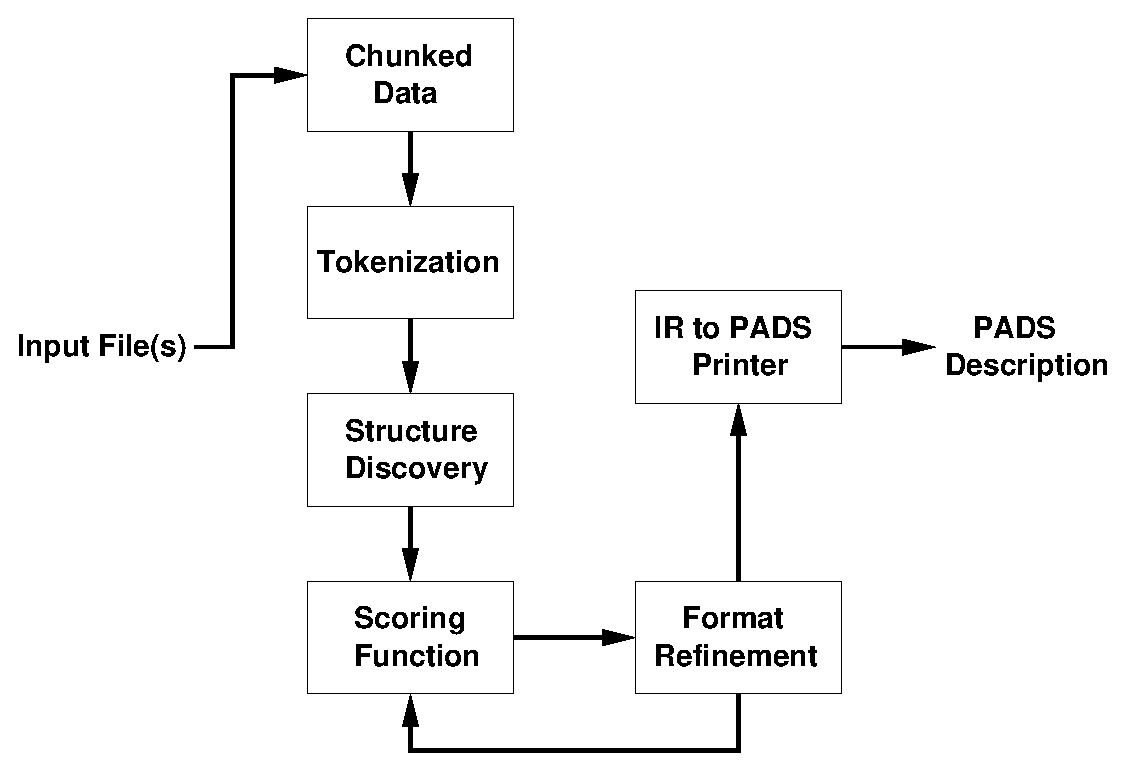
\epsfig{file=archi.eps, width=.9\columnwidth}
\caption{Architecture of the format inference engine}
\vspace*{-5mm}
\label{fig-archi}
\end{center}
\end{figure}

Figure \ref{fig-archi} gives an overview of our format inference
architecture. The input data, or ``training set,'' is first
``chunked'' into records where each record is a piece of recurrent
data such as a line, a paragraph, or a file (if the input consists of
multiple files).  The user specifies the unit of repetition when
invoking our learning tool.  Each record is then broken down into a
series of tokens where each token can be a punctuation symbol, a
number, a date, a time, or a number of other basic types.  Our
learning system has a basic tokenization scheme skewed toward systems
data, but users may specify a different scheme for their own domain
through a configuration file.  For example, computational biologists
may want to specify new base types for DNA strings or other common
recurring patterns.

In the structure discovery phase, we use a top-down, divide-and-conquer
scheme inspired in part by the work of Arasu on
information extraction from web pages~\cite{arasu+:sigmod03}. 
When a type constructor has been chosen, the data is partitioned accordingly
and the algorithm recursively analyzes subparts.  This
rough structure is represented in an intermediate representation (IR)
that has similar expressive power to the \pads{} language. 
The format refinement phase analyzes the IR produced by structure discovery
and repeatedly applies rewrite rules.  
In effect, this refinement phase is equivalent to a greedy, local search
procedure aimed at improving the quality of the inferred format.

\subsection {Chunking and Tokenization}

\begin{figure}
\begin{center}
\begin{tabular}{|l|l|}
\hline
Name   &  Description               \\ \hline\hline
Pint  &   Integer \\ 
Palpha & Alpha-numeric string including '$\_$' and '$-$' \\
Pip & IP address \\
Pemail & Email address \\
Pmac & Mac address \\
Pdate & Simple date format \\
Ptime & Simple time format \\
Ppath & File system path \\
Phostname & Hostname \\
Purl  & URL \\
PbXML & Beginning XML tag \\
PeXML & Ending XML tag \\
Pother & Punctuation character \\\hline
\end{tabular}

\caption{Basic token types in default configuration.}
\label{figure:base-types}
\end{center}
\end{figure}
 



    *  mention system parameterization for multiple tokenizations for different domains
    * mention current skew towards systems data
    * ignore problems in this section -- save that for discussion/future work section
    * mention stream of tokens generated for running example 

\subsection {Structure Discovery}

    *  role = quickly find a description in the "approximate area" of the correct description
    * explain structure of a generic "top-down" inference algorithm -- perhaps give pseudocode
    * explain our heuristics: generation of histograms, choice of struct, array, union, base type
    * grouping construct (introduce additional example as needed)
    * show (part of?) description of running example 

\subsection {Information-Theoretic Scoring}

    *  role = evaluate the "goodness" of the description relative to data
    * explain the information-theoretic principles
    * give the formulas 

\subsection {Structure Refinement}

    *  role = starting with the candidate structure, search for nearby descriptions that optimize an information theoretic scoring function
    * explain the 3 parts: value independent, value dependent, value independent
    * give (partial) list of rules used -- we need to work on notation for explaining these rules
    * illustrate several transformations using the running example
    * compare example after rewriting to the example from subsection 3.4 above
    * optional subsubsection: theory suggesting our algorithm is "correct" (we'd need a semantics for our IR then) 

\subsection {Finishing Up}

    * printing pads syntax and invoking toolchain

\section {Discussion}
\label{sec:discussion}
\subsection{Related Work}

\subsection {Current and Future Work}

thoughts on problems with tokenization; information theory; partial
descriptions; user interface; recursion; more experimentation with a
broader range of formats



\section{Conclusions}
\section{Conclusion} 
\label{sec:conclusion}

Ad hoc data is pervasive and valuable: in industry, in medicine, and
in scientific research.  Such data tends to have poor documentation,
to contain various kinds of errors, and to be voluminous.  Unlike
well-behaved data in standardized relational or \xml{} formats, such
data has little or no tool support, forcing data analysts and
scientists to waste valuable time writing brittle custom code, even if
all they want to do is convert their data into a well-behaved format.
To improve the situation, various researchers have developed data
description languages such as \pads{}, \datascript{}, and
\packettypes{}.  Such languages allow analysts to write terse,
declarative descriptions of ad hoc data.  A compiler then generates a
parser and customized tools.  Because these languages are tailored to
their domain, they can provide useful services automatically while a
more general purpose tool, such as \lex{}/\yacc{} or \perl{}, cannot.

In the spirit of Landin, we have taken the first steps toward
specifying a semantics for this class of languages by defining the
data description calculus \ddc{}.  This calculus, which is a dependent
type theory with a simple set of orthogonal primitives, is expressive
enough to describe the features of \pads{}, \datascript{}, and
\packettypes{}.  In keeping with the spirit of the data description
languages, our semantics is transformational: instead of simply
recognizing a collection of input strings, we specify how to transform
those strings into canonical in-memory representations annotated with
error information.  Furthermore, we prove that the error information
is meaningful, allowing analysts to rely on the error summaries rather
than having to re-vet the data by-hand.

We have already used the semantics to identify bugs in the
implementation of \padsc{} and to highlight areas where \padsc{}
sacrifices safety for speed.  We have also used the semantics as a guide
for the design of a whole new language, \padsml{}, designed
specifically for functional programmers.  In the future, we hope 
\ddc{} will serve as a solid foundation for the next 700 data 
description languages to come.


\section*{Acknowledgments}

Our work benefited greatly from thoughts and comments by
Alex Aiken, David Blei, David Burke, John Launchbury, Chris Ramming, 
and Vikas ...

This material is based upon work 
supported by DARPA under grant FA8750-07-C-0014
and the NSF
   under grants 0612147 and 0615062.
Any opinions, findings, and conclusions or recommendations
   expressed in this material are those of the authors and do not
   necessarily reflect the views of DARPA or the NSF.

\bibliographystyle{abbrv}
\bibliography{pads}

\appendix
\section{Language Syntax}
{\allowdisplaybreaks
\noindent
{\bf Syntax of data descriptions and other types}
\label{app:syntax-dd}
\begin{bnf}
\name{Constants} \meta{k} \::= \mcd{true} \| \mcd{false} \| \mcd{()} \| ...
\\
\name{Type Variables} \meta{\alpha}
\\
\name{Type Names} \meta{t}
\\
\name{\Core{} Types} \meta{T} \::= 
  \alpha 
\| {Pbase} 
\| M 
\nlalt \ppair x {T_1} {T_2} 
\| \precord {\nont{ffts}} 
\| \nont{tas}\;t(M) 
\nlalt \pset x T M 
\nlalt \parray T {M_{sep}} {M_{term}} 
\\
\name{\Core{} Datatypes} \meta{D} \::= 
  \mcd{datatype}\; \nont{tps}\; t(x{:}F) = \nont{b} \nlalt
  \mcd{type}\; \nont{tps}\; t(x{:}F) = T
\\
\name{Type Parameters} \meta{tps} \::= \cdot \| \alpha \| (\nont{tvs})
\\
\name{} \meta{tvs} \::= \alpha \| \alpha,\, \nont{tvs}
\\
\name{Type Arguments} \meta{tas} \::= \cdot \| T \| (\nont{ts})
\\
\name{} \meta{ts} \::= T \| T,\, \nont{tss}
\\
\name{} \meta{b} \::= \nont{cs} \| \mcd{case}\; M\; \mcd{of}\; \nont{ccs}
\\
\name{} \meta{cs} \::= c\;\mcd{of}\;T \| c\;\mcd{of}\;T \cvb \nont{cs}
\\
\name{} \meta{ccs} \::= 
  \nont{pat} \Rightarrow c\;\mcd{of}\;T \nlalt
  \nont{pat} \Rightarrow c\;\mcd{of}\;T \cvb \nont{ccs}
\\
\name{\Core{} Field Types} \meta{ffts} \::= \nont{fft} \| \nont{fft};\;\nont{ffts}
\\
\name{\Core{} Field Type} \meta{fft} \::= T \| x = T
\end{bnf}
%\begin{bnf}
\name{Constants} \meta{k} \::= \mcd{true} \| \mcd{false} \| \mcd{()} \| ...
\\
\name{Type Variables} \meta{\alpha}
\\
\name{Type Names} \meta{t}
\\
\name{\Core{} Types} \meta{T} \::= 
  \alpha 
\| {Pbase} 
\| M 
\nlalt \ppair x {T_1} {T_2} 
\| \precord {\nont{ffts}} 
\| \nont{tas}\;t(M) 
\nlalt \pset x T M 
\nlalt \parray T {M_{sep}} {M_{term}} 
\\
\name{\Core{} Datatypes} \meta{D} \::= 
  \mcd{datatype}\; \nont{tps}\; t(x{:}F) = \nont{b} \nlalt
  \mcd{type}\; \nont{tps}\; t(x{:}F) = T
\\
\name{Type Parameters} \meta{tps} \::= \cdot \| \alpha \| (\nont{tvs})
\\
\name{} \meta{tvs} \::= \alpha \| \alpha,\, \nont{tvs}
\\
\name{Type Arguments} \meta{tas} \::= \cdot \| T \| (\nont{ts})
\\
\name{} \meta{ts} \::= T \| T,\, \nont{tss}
\\
\name{} \meta{b} \::= \nont{cs} \| \mcd{case}\; M\; \mcd{of}\; \nont{ccs}
\\
\name{} \meta{cs} \::= c\;\mcd{of}\;T \| c\;\mcd{of}\;T \cvb \nont{cs}
\\
\name{} \meta{ccs} \::= 
  \nont{pat} \Rightarrow c\;\mcd{of}\;T \nlalt
  \nont{pat} \Rightarrow c\;\mcd{of}\;T \cvb \nont{ccs}
\\
\name{\Core{} Field Types} \meta{ffts} \::= \nont{fft} \| \nont{fft};\;\nont{ffts}
\\
\name{\Core{} Field Type} \meta{fft} \::= T \| x = T
\end{bnf}
%%% Local Variables: 
%%% mode: latex
%%% TeX-master: "paper"
%%% End: 


\noindent
{\bf Syntax of terms}
\label{app:syntax-terms}
\begin{bnf}
\name{Types} \meta{F} \::= 
  T           \descr{type of \pvalue{}} 
\nlalt \nont{base} \descr{values of ordinary base types} 
\nlalt \mcd{PD}    \descr{PD type}
\nlalt F * F       \descr{ordinary pairs} 
\nlalt \{\nont{fts}\}     \descr{ordinary records} 
\nlalt F \-> F     \descr{functions}
\nlalt \pstream F  \descr{streams}
\\
\name{Field Types} \meta{fts} \::= x = F \| x=F,\;\nont{fts}
\\
%\end{bnf}
%\begin{bnf}
\name{Parse Descriptors} \meta{pd} \::=   
  G \| B \| N \| S \| U
\\
\name{\Core{} Terms} \meta{N} \::=  
       Pbase[M_1](M_2)                \descr{base type constructor}
\nlalt \langle M \rangle              \descr{unit value (with singleton type M)}
\nlalt (x{=}{M_1} \mathrel{**} {M_2}) \descr{pair}
\nlalt \lcr \nont{fs} \rcr            \descr{record}
\nlalt c[M_1](M_2)                    \descr{data type constructor}
\nlalt \{x = {M_1} \cvb {M_2}\}       \descr{constrained type, with
  $M_2$ the constraint}
\nlalt \mcd{Parray}(M, M_{sep}, M_{term})   \descr{array; first element is stream}
\end{bnf}

\newpage

\begin{bnf}
\name{Terms} \meta{M} \::= 
       x                        \descr{variable}
\nlalt N                        \descr{\core{} terms}
\nlalt k                        \descr{constants}
\nlalt \nont{pd}                      \descr{pd value}
\nlalt (M_1 * M_2)              \descr{ordinary pair}
\nlalt \{\nont{fs}\}        \descr{ordinary record}
\nlalt \tfun {x_1}{x_2}{F_1}{F_2}{M}     \descr{recursive function x1 with arg x2}
\nlalt \mcd{nil}                \descr{empty stream}
\nlalt M_1 \mathrel{::} M_2     \descr{cons}
\nlalt \mcd{case}\;M\;\mcd{of}\;\nont{ms} \descr{deconstructors}
\nlalt M_1\;(M_2)               \descr{function application}
\nlalt \mcd{op}\;M                     \descr{additional uninteresting operations}
\nlalt \mcd{let}\;x = M_1\;\mcd{in}\;M_2           \descr{computation in host language}
\nlalt \mcd{cast}\;(M : T)             \descr{type annot/dependent cast?}
\\
\name{Fields} \meta{fs} \::= x = M \| x = M; \nont{fs}
\\
\name{Matches}\meta{ms} \::= 
  \nont{pat} \Rightarrow M \| \nont{pat} \Rightarrow M \cvb \nont{ms}
\end{bnf}
%{\small
\begin{verbatim}
M ::=  x                        // variable
     | Pbase[M1](M2)            // base type constructor; M1 is
                                   an argument to the type; M2 computes the rep)
     | c(M)                     // data type constructor with parameter M
     | (x:M1 ** M2)             // pair
     | {fields}                 // record
     | {x = M1 | M2}            // set-type; M2 is the predicate
     | Parray(M, Msep, Mterm)   // array; first element is stream
     | k                        // constants
     | let x = M in M           // computation in host language
     | <M>                      // unit value given singleton type M
     | (M1 * M2)                // ordinary pair
     | nil                      // empty list
     | M1 :: M2                 // cons
     | case M of MS             // deconstructors
     | fun x1(x2:F1):F2 = M     // recursive function x1 with arg x2
     | M1 (M2)                  // function application
     | cast (M : T)             // type annot/dependent cast?
     | op M                     // additional uninteresting operations
     
fields ::= x = M | x = M; fields

pd ::=   G    // good
     |   B    // bad
     |   N    // nested error
     |   S    // semantic error
     |   U    // unknown
\end{verbatim}
}

  
\newpage

\noindent
{\bf Syntax of patterns}
\label{app:syntax-pat}
\begin{bnf}
% \name{Parse Descriptors} \meta{pd} \::=   
%          G    \descr{good}
% \nlalt   B    \descr{bad}
% \nlalt   N    \descr{nested error}
% \nlalt   S    \descr{semantic error}
% \nlalt   U    \descr{unknown}
\name{\Core{} Patterns} \meta{fpat} \::=
x \| \nont{Pbase}(\nont{pat})
\nlalt \langle \nont{pat} \rangle             \descr{singleton}
\nlalt (\nont{fpat} \mathrel{**} \nont{fpat})   \descr{\core{} pair}
\nlalt \lcr \nont{ffps} \rcr                  \descr{\core{} record}
\nlalt c(\nont{fpat})                          \descr{constructor}
\nlalt \{\nont{fpat} \cvb \nont{cpat}\}        \descr{type constaint}
\nlalt \mcd{Parray}(\nont{pat}, x_{sep}, x_{term}) \descr{array with stream, sep and term.}
\nlalt \nont{fpat}\langle\langle\nont{pdpat}\rangle\rangle
\\
\name{Patterns}\meta{pat} \::= 
       \nont{fpat} \descr{\core{} pattern}
\nlalt k \| \nont{pdpat}                      \descr{constants and parse descriptors}
\nlalt (\nont{pat} * \nont{pat})              \descr{normal pair}
\nlalt \{\nont{fps}\}                        \descr{record}
\nlalt \mcd{nil} \| \nont{pat}_1 \mathrel{::} \nont{pat}_2 \descr{stream}
\\
\name{\Core{} Field Pattern} \meta{ffps} \::= x = \nont{fpat} \| x = \nont{fpat};\;\nont{ffps}
\\
\name{Constraint Pattern} \meta{cpat} \::= x \| \mcd{true} \| \mcd{false}
\\
\name{PD Pattern} \meta{pdpat}\::= x \| \nont{pd}
\\
\name{Field Pattern} \meta{fps} \::= x = \nont{pat} \| x = \nont{pat};\;\nont{fps}
\end{bnf}
%{\small
\begin{bnf}
% \name{Parse Descriptors} \meta{pd} \::=   
%          G    \descr{good}
% \nlalt   B    \descr{bad}
% \nlalt   N    \descr{nested error}
% \nlalt   S    \descr{semantic error}
% \nlalt   U    \descr{unknown}
\name{\Core{} Patterns} \meta{fpat} \::=
x \| \nont{Pbase}(\nont{pat})
\nlalt \langle \nont{pat} \rangle             \descr{singleton}
\nlalt (\nont{fpat} \mathrel{**} \nont{fpat})   \descr{\core{} pair}
\nlalt \lcr \nont{ffps} \rcr                  \descr{\core{} record}
\nlalt c(\nont{fpat})                          \descr{constructor}
\nlalt \{\nont{fpat} \cvb \nont{cpat}\}        \descr{type constaint}
\nlalt \mcd{Parray}(\nont{pat}, x_{sep}, x_{term}) \descr{array with stream, sep and term.}
\nlalt \nont{fpat}\langle\langle\nont{pdpat}\rangle\rangle
\\
\name{Patterns}\meta{pat} \::= 
       \nont{fpat} \descr{\core{} pattern}
\nlalt k \| \nont{pdpat}                      \descr{constants and parse descriptors}
\nlalt (\nont{pat} * \nont{pat})              \descr{normal pair}
\nlalt \{\nont{fps}\}                        \descr{record}
\nlalt \mcd{nil} \| \nont{pat}_1 \mathrel{::} \nont{pat}_2 \descr{stream}
\\
\name{\Core{} Field Pattern} \meta{ffps} \::= x = \nont{fpat} \| x = \nont{fpat};\;\nont{ffps}
\\
\name{Constraint Pattern} \meta{cpat} \::= x \| \mcd{true} \| \mcd{false}
\\
\name{PD Pattern} \meta{pdpat}\::= x \| \nont{pd}
\\
\name{Field Pattern} \meta{fps} \::= x = \nont{pat} \| x = \nont{pat};\;\nont{fps}
\end{bnf}
}

%%% Local Variables: 
%%% mode: latex
%%% TeX-master: "paper"
%%% End: 


\noindent
{\bf Syntax of programs}
\label{app:syntax-prog}
\begin{bnf}
\name{Program} \meta{prog} \::= 
  M              
 \nlalt D\; \nont{prog}          \descr{type declaration}
 \nlalt \mcd{val}\;x = M\;\mcd{prog} \descr{value declaration}
\end{bnf}
%{\small
\begin{verbatim}
prog ::= M              
       | D prog          // type declaration
       | val x = M prog  // value declaration
\end{verbatim}
}

}
%%% Local Variables: 
%%% mode: latex
%%% TeX-master: "paper"
%%% End: 


\end{document}

%%% Local Variables:
%%% mode: outline-minor
%%% End:

